\lstset{frame=single,
  basicstyle=\footnotesize ,
  backgroundcolor=\color{white},
  language=Python}

\section{The PyUtilib Component Architecture}

\label{chap:pca}

The PyUtilib Component Architecture (\pca) is included in the
PyUtilib software package~\cite{PyUtilib}.  It inspired by the Trac
plugin framework~\cite{Trac}, and it was initially motivated by our
need for an independent, self-contained plugin framework for
scientific computing applications.  The core of the \pcasp is
provided through a small set of classes within PyUtilib's
\code{pyutilib.component.core} package.  This section provides a
tutorial introduction of the \pcasp as well as a detailed description
of the \pcasp classes and their functionality.


\subsection{\pcasp Definitions}

There are different notions of software components~\cite{Mar05}, so we begin by
providing some definitions.  The relationships among these terms is
illustrated in Figure \ref{fig:defs}.  A \textit{plugin} is a
class that implements a set of related methods in the context of an
application.  Thus, a plugin can be described as a component definition.

An \textit{interface} class defines a type that a plugin uses to register
its capabilities.  A plugin class includes declarations that denote that
it implements one-or-more interfaces. An interface is defined by the
methods and data that are used.  However, the \pcasp does not enforce
this interface or support interface conversions (see Zope~\cite{Zope}
and Envisage~\cite{Envisage} for examples of plugin frameworks that
support this functionality).

A \textit{service} is an instance of a plugin class that is registered
globally with its interfaces.  We say that a plugin class instance
is \textit{active} if it is registered, and a plugin class instance
is only treated as a service if it is active.  A service can be an
instance of either a singleton or non-singleton plugin. There is
exactly one service for a singleton plugin (and that service is
instantiated automatically), whereas there can be multiple services
of non-singleton plugins.  Singleton plugins are active by default,
whereas non-singleton plugins are conditionally active depending
how the plugin interface is declared.

\begin{figure}[htb]
  \center
  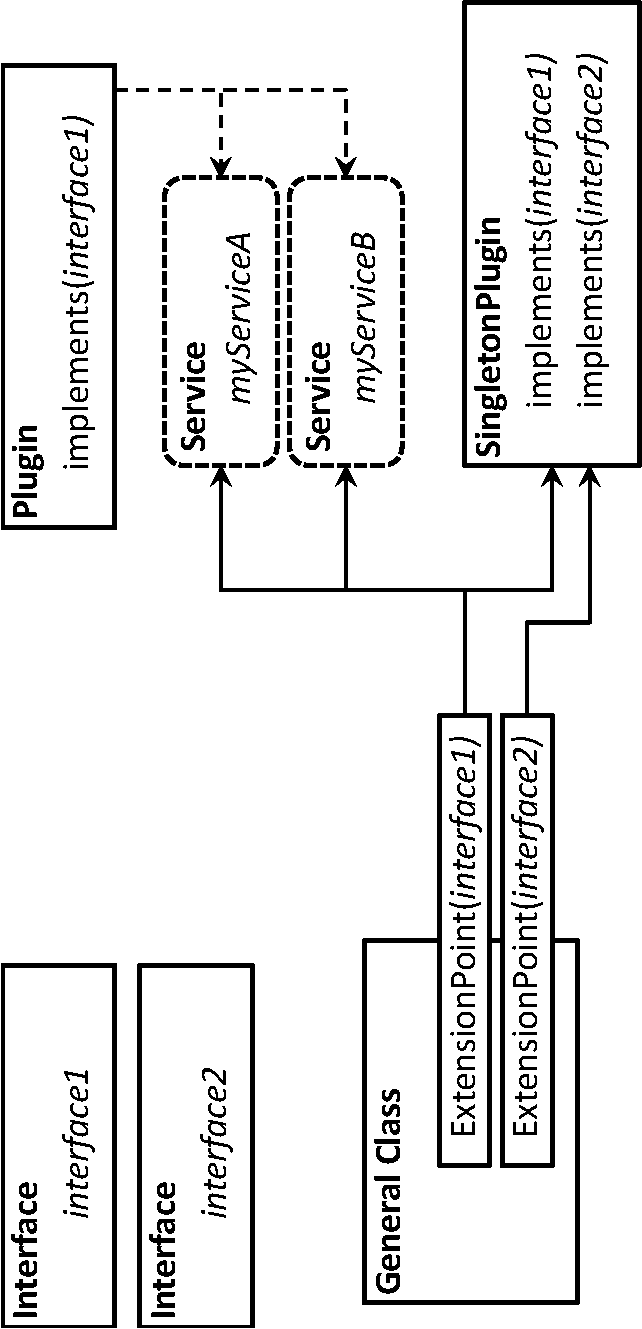
\includegraphics[height=5in,angle=-90]{figures/definitions.pdf}
  \caption{An illustration of how classes within the PCA relate to one another.  Interface classes are independent declarations of APIs.  Plugin classes can declare that they implement an Interface's API, and extension points declare that they require a specific
Interface API.  Both singleton and non-singleton plugins can be used, but services for non-singleton plugins are explicitly constructed.}
  \label{fig:defs}
\end{figure}

A software application or a component can declare \textit{extension
points} that other components can \textit{plug in} to. An extension
point is defined with respect to a specific \textit{interface}
class.  Thus, a service that supports an interface plugs into an
extension point for that interface.  In this way, extension points
provide a generic mechanism for applications to employ the functionality
provided by other services.

This mechanisms supports a flexible,
modular programming paradigm that enables software applications to
be extended in a dynamic manner.  The \pcasp includes a global component
registry and a framework for automating the execution of plugin
services.  All plugins and interfaces automatically register themselves
with the registry.  This registry then acts as a broker, dynamically providing
extension points with the appropriate matching services at run time.  
Thus, an application
developer can define extension points without knowing how they will be
implemented, and plugin developers can register extensions without
needing to know the details of how -- or where -- they are employed.
This capability facilitates the dynamic registration
and application of components within large software systems.

\subsubsection{Relationship to the Trac Component System}

The general design of \pcasp is inspired by the plugin system
included in Trac~\cite{Trac}. The \pcasp generalizes the Trac
component architecture by supporting namespace management of plugins,
non-singleton plugins, support for non-active plugin instances and
caching of interface interactions. For those familiar with Trac,
the following classes roughly correspond with each other:
\begin{center}
\begin{tabular}{|l|l|} \hline
    Trac Class Name &   PyUtilib Class Name \\ \hline
    Interface   & Interface \\
    ExtensionPoint  & ExtensionPoint \\
    Component   & SingletonPlugin \\
    ComponentManager    & PluginEnvironment \\ \hline
\end{tabular}
\end{center}
The \code{PluginEnvironment} class is used to manage plugins, but unlike Trac this class does not   need to be explicitly constructed.


\subsection{A Simple Example}

Figure~\ref{fig:example1} provides a simple example that is adapted from
the description of the Trac component architecture~\cite{TCA}. This
example illustrates the three main steps to setting up a plugin: 
\begin{enumerate}
\item Defining an interface
\item Declaring extension points
\item Defining classes that implement the interface. 
\end{enumerate}
This example begins by defining \code{ITaskObserver}, a subclass of \code{Interface}. 
Although it is not required to define methods in an interface, these
declarations provide documentation for plugin developers.
We then declare a \code{TaskList} that manages a
dictionary of tasks and descriptions.  The \code{TaskList} creates an
\code{ITaskObserver} extension point, and when a task is added to the
task list, it calls all services that implement the \code{ITaskObserver}
interface.  Finally, we define a \code{TaskPrinter} as a singleton
plugin.  The \code{TaskPrinter} implements the \code{ITaskObserver}
interface, and when called prints the task name and description.  As the
\code{TaskPrinter} is a singleton plugin, the \pcasp automatically
instantiates and registers a single \code{TaskPrinter} service.

%In this example, a singleton plugin is declared, which automatically
%registers the single component service. Non-singleton plugin services need to
%explicitly created, but they are also automatically registered. 


Assuming the module in Figure~\ref{fig:example1} 
is saved as \code{task.py}, then the following Python script 
illustrates how this plugin is used:
\begin{quotation}
\begin{lstlisting}
from task import *

# Construct a TaskList object and then add several tasks.
task_list = TaskList()
task_list.add('Make coffee', 'Need to make some coffee')
task_list.add('Bug triage', 'Double-check all issues')
\end{lstlisting}
\end{quotation}
This script generates the following output:
\begin{quotation}
\begin{lstlisting}
Task: Make coffee
      Need to make some coffee
Task: Bug triage
      Double-check all issues
\end{lstlisting}
\end{quotation}


\begin{figure}
\center
\begin{quotation}
\begin{lstlisting}
# A simple example that manages a task list.  An observer 
# interface adds actions that occur when a task is added.
from pyutilib.component.core import *

# An interface class that defines the API for plugins that
# observe when a task is added.
class ITaskObserver(Interface):

    def task_added(name, description):
        """Called when a task is added."""

# The task list application, which declares an extension point
# for observers.  Observers are notified when a new task
# is added to the task list.
class TaskList(object):
    observers = ExtensionPoint(ITaskObserver)

    def __init__(self):
        """The TaskList constructor, which initializes the list"""
        self.tasks = {}

    def add(self, name, description):
        """Add a task, and notify the observers"""
        self.tasks[name] = description
        for observer in self.observers:
            observer.task_added(name, description)

# A plugin that prints information about tasks when they
# are added.
class TaskPrinter(SingletonPlugin):
    implements(ITaskObserver)

    def task_added(self, name, description):
        print 'Task:', name
        print '     ', description
\end{lstlisting}
\end{quotation}
\caption{A simple example of \pcasp components.}
\label{fig:example1}
\end{figure}



\section{PCA Classes}
\label{chap:core}

The \pcasp consists of the following core classes that are defined in the \code{pyutilib.component.core} package:
\begin{description}
\item[Interface] Subclasses of this class declare plugin interfaces that are registered in the \pca. 
\item[ExtensionPoint] A class used to declare extension points, which can access services with a particular interface.
\item[Plugin] Subclasses of this class declare plugins, which can be used to implement interfaces within the \pca. 
\item[SingletonPlugin] Subclasses of this class declare singleton plugins, for which a single service is constructed. 
\item[PluginEnvironment] A class that maintains the registries for interfaces, extension points, plugins and services. 
\item[PluginGlobals] A class that maintains global data concerning the set of environments that are currently being used. 
\item[PluginError] The exception class that is raised when errors arise in the \pca. 
\end{description}
The following sections provide a detailed description of how these classes are used in the
\pca.

\subsection{Interfaces and Extension Points}

A subclass of the \code{Interface} class is used to declare extension
points in an application. The \code{ExtensionPoint} class is used to
declare an extension point and to retrieve information about the plugins
that implement the specified interface. For example, the following is
a minimal declaration of an interface and extension point:
\begin{quotation}
\begin{lstlisting}
class IMyInterface(Interface):
   """An interface subclass"""

ep = ExtensionPoint(IMyInterface)
\end{lstlisting}
\end{quotation}
Note that the \code{IMyInterface} class is not required to define the API
of the interface. The \pcasp does not enforce checking of API conformance
for plugins, and hence any declaration in the \code{IMyInterface}
class would be ignored. Additionally, note that an instance of
\code{IMyInterface} is not created; the \code{IMyInterface} class is simply
used to declare a type that is used to index related plugins.

An instance of \code{ExtensionPoint} can be used to iterate through
all extensions, or to search for an extension that matches a particular
keyword. For example, the following code iterates through all extensions
and applies the \code{pprint} method:
\begin{quotation}
\begin{lstlisting}
for service in ep:
  service.pprint()
\end{lstlisting}
\end{quotation}
If you wish to know the number of services that are registered with an
extension point, you can call the standard \code{len} function:
\begin{quotation}
\begin{lstlisting}
print len(ep)
\end{lstlisting}
\end{quotation}

Several other methods can be used to more carefully select services from
an extension point. The \code{extensions} method returns a Python \code{set} object
that contains the services:
\begin{quotation}
\begin{lstlisting}
#
# This loop iterates over all services, just the same
# as when an the iterator method is used (see above).
#
for service in ep.extensions():
  service.pprint()
\end{lstlisting}
\end{quotation}
The Python \code{\_\_call\_\_} method provides a convenient shorthand for this same function.  Thus, the following is equivalent:
\begin{quotation}
\begin{lstlisting}
for service in ep():
  service.pprint()
\end{lstlisting}
\end{quotation}

These methods have two optional arguments that control the selection of services.  The \code{all} 
keyword indicates whether
the set returned by \code{extensions} includes all disabled services. 
\begin{quotation}
\begin{lstlisting}
#
# This loop iterates over all services, including
# the 'disabled' services.
#
for service in ep.extensions(all=True):
  service.pprint()
\end{lstlisting}
\end{quotation}
It is
convenient to explicitly support enabling and disabling services in many
applications, though services are enabled by default. Disabled services
remain in the registry, but by default they are not included in the set
returned by an extension point.

The \pcasp can also support \textit{named services}, which requires that
the services have a \code{name} attribute. Service names are not required
to be unique. For example, when multiple instances of a non-singleton
plugin are created, then these services can be accessed as follows:
\newpage
\begin{quotation}
\begin{lstlisting}
#
# A simple plugin that implements the IMyInterface interface
#
class MyPlugin(Plugin):
  implements(IMyInterface)

  def __init__(self):
      self.name="myname"

#
# Another simple plugin that implements the IMyInterface interface
#
class MyOtherPlugin(Plugin):
  implements(IMyInterface)

  def __init__(self):
      self.name="myothername"

#
# Constructing services
#
service1 = MyPlugin()
service2 = MyPlugin()
service3 = MyOtherPlugin()

#
# A function that iterates over all IMyInterface services, and
# returns the MyPlugin instances (which are service1 and service2).
#
def get_services():
    ep = ExtensionPoint(IMyInterface)
    return ep("myname")
\end{lstlisting}
\end{quotation}
In some applications, there is a one-to-one correspondence between service
names and their instances. In this context, a simpler syntax is to use
the \code{service} method:
\begin{quotation}
\begin{lstlisting}
class MySingletonPlugin(SingletonPlugin):
  implements(IMyInterface)

  def __init__(self):
      self.name="mysingletonname"

ep = ExtensionPoint(IMyInterface)
ep.service("mysingletonname").pprint()
\end{lstlisting}
\end{quotation}
The \code{service} method raises a \code{PluginError} if there is more than one service
with a given name. Note, however, that this method returns \code{None} if no
service has been registered with the specified name.

Note that an integer cannot be used to select a service from an extension
point. Services are not registered in an indexable array, so this option
is disallowed.


\subsection{Plugins}

\pcasp plugins are subclasses of either the \code{Plugin} or \code{SingletonPlugin}
classes. Subclasses of \code{Plugin} need to be explicitly constructed,
but otherwise they do not need to be registered; simply constructing a
subclass of \code{Plugin} invokes the registration of that instance. Similarly,
simply declaring a subclass of \code{SingletonPlugin} invokes both the construction
and registration of this component.

\pcasp plugins are registered with different interfaces using the \code{implements}
function, which is a static method of \code{Plugin}. Note that a plugin can be
registered with more than one interface. Further, a service can be applied to different
extension points independently, but it can maintain state information
that impacts its use across different extension points.

The default behavior of the \pcasp is to ignore the declarations in an interface class, but
the \code{implements} function includes an \code{inherit} keyword can be used to define a plugin that 
inherits interface methods.  For example:
\begin{quotation}
\begin{lstlisting}
class IMyInterface(Interface):
    def print(self):
        print "This is the default print method"

    def add(self, x):
        return x+2

class MyPlugin(Plugin):
    implements(IMyInterface, inherit=True)

    def add(self, x):
        return x+3
\end{lstlisting}
\end{quotation}
In this example, the \code{MyPlugin} class implements the \code{IMyInterface} interface.  Since the \code{inherit} keyword is \code{True}, the \code{MyPlugin} class inherits the \code{print} method.  Thus, \code{MyPlugin} has a complete implementation of the \code{IMyInterface} interface.

Although this behavior is generally useful, the API for \pcasp
intentionally does not make interface inheritance the default behavior.
When inheritance is used, a developer can get into trouble if they mistype
the name of a plugin method.  When this occurs, the interface method is
used, without any notification to the user.  This could easily lead to
erroneous plugin behavior that is quite difficult to track down.

When \code{Plugin} classes are instantiated or \code{SingletonPlugin}
classes are declared, the resulting class service is registered in global \pcasp
data (see below).  The \code{Plugin} class includes several methods
for controlling this registration.  The \code{disable} and \code{enable}
methods provide a simple mechanism for controlling whether a service
is returned with associated extension points.  These methods clear the
\pcasp caches that are associated with these extension points to ensure
that the extension points are correctly setup.  The \code{activate}
and \code{deactivate} methods respectively add and remove the service
from the global environment.  This has a similar effect as \code{enable}
and \code{disable}, except that after deactivation the service is no
longer associated with the \pcasp global data, while after \code{disable}
the service is still registered but flagged as not active.


\subsection{Environments}

The \code{PluginEnvironment} class defines namespaces that contain component services and interfaces.
These namespaces provide
a mechanism for organizing component services in an extensible
manner. Applications can define new namespaces that contain their services
without worrying about conflicts with services defined in other Python
libraries.

A global registry of environments
is maintained by the \code{PluginGlobals} class. This registry is a stack
of environments, and the top of this stack defines the current
environment. When an interface is declared, its namespace is the name
of the current environment. For example:
\begin{quotation}
\begin{lstlisting}
#
# Declare an interface in the current environment
#
class Interface1(Interface):
   pass

#
# Set the current environment to 'new_environ'
#
PluginGlobals.push_env( "new_environ" )

#
# Declare an interface in the 'new_environ' environment
#

class Interface2(Interface):
   pass

#
# Go back to the original environment
#
PluginGlobals.pop_env()
\end{lstlisting}
\end{quotation}
Component services are automatically registered in namespaces in two ways.  First,
for each interface that the service implements, the service is registered in 
the namespace in which the interface was declared.  Second, a service is 
registered in the namespace in which its corresponding plugin class is declared.

For example, consider the code in Figure~\ref{fig:env1}.
When \code{Plugin1} is instantiated, this service is registered in the 
following environments:
\begin{quotation}
\begin{lstlisting}
env1 for Interface1
env2 for Interface2
env4 for Interface1
env3
\end{lstlisting}
\end{quotation}
The last registration is the default, since a service is always
registered in the environment where its plugin class is declared.
Note that \code{env4} namespace is declared explicitly in this example.


\begin{figure}
\begin{quotation}
\begin{lstlisting}
#
# Declare Interface1 in namespace env1
#
PluginGlobals.push_env("env1")

class Interface1(Interface):
   pass

#
# Declare Interface2 in namespace env2
#
PluginGlobals.push_env("env2")

class Interface2(Interface):
   pass

PluginGlobals.pop_env()

#
# Declare Plugin1 in namespace env3
#
PluginGlobals.push_env("env3")

class Plugin1(Plugin):

   implements(Interface1)
   implements(Interface2)
   implements(Interface1,"env4")

PluginGlobals.pop_env()
\end{lstlisting}
\end{quotation}
\caption{\label{fig:env1} Illustration of how plugin declarations are related to component environments.}
\end{figure}


\subsection{Global Component Data}

Global component data in \pcasp is managed in the \code{PluginGlobals} class. This
class contains a variety of static methods that are used to access
this data:
\begin{description}
\item[default\_env] This method returns the default environment, which is constructed when the \pcasp is loaded. 
\item[env] This method returns the current environment if no argument is specified. Otherwise, it returns the specified environment. 
\item[push\_env,pop\_env] These methods respectively push a new environment onto the environment stack and pop the current environment from the stack. 
\item[services] This method returns the component services in the current environment (or the named environment if one is specified). 
\item[singleton\_services] This method returns the singleton component services in the current environment (or the named environment if one is specified). 
\item[load\_services] Load services using \code{IPluginLoader} extension points (see Section~\ref{sec:loaders}). 
\item[pprint] This method provides a text summary of the registered interfaces, plugins and services. 
\item[clear] This method empties the environment stack and defines a new default environment. This setup then bootstraps the configuration of the \code{pyutilib.component.core} environment. Note that this does not clear the component registry; in practice that may not make sense since it is not easy to reload modules in Python. 
\end{description}




